\section{Cel dokumentu}
\suppressfloats[t]

Niniejszy dokument powstał w celu przedstawienia wszystkich poziomów uprawnień które znajdą się w Systemie Obsługi Konferencji (SOK), oraz akcji (przypadków użycia) jakie użytkownik o danym zakresie uprawnień może wykonać w systemie. 

\section{Dokumentyi pliki powiązane}

\begin{itemize}
  \item \textit{administrator.vsdx} - dokument przypadków użycia użytkownika ADMINISTRATOR (plik programu Microsoft Visio 2013)
  \item \textit{administrator.jpg} - wyeksportowany dokument przypadków użycia użytkownika ADMINISTRATOR
  \item \textit{pracownik.vsdx} - dokument przypadków użycia użytkownika PRACOWNIK (plik programu Microsoft Visio 2013)
  \item \textit{pracownik.jpg} - wyeksportowany dokument przypadków użycia użytkownika PRACOWNIK
  \item \textit{rodzina.vsdx} - dokument przypadków użycia użytkownika RODZINA PRACOWNIKA (plik programu Microsoft Visio 2013)
  \item \textit{rodzina.jpg} - wyeksportowany dokument przypadków użycia użytkownika RODZINA PRACOWNIKA 
  \item \textit{rodzina.vsdx} - dokument przypadków użycia użytkownika RODZINA PRACOWNIKA (plik programu Microsoft Visio 2013)
  \item \textit{rodzina.jpg} - wyeksportowany dokument przypadków użycia użytkownika RODZINA PRACOWNIKA 
  \item \textit{recenzent.vsdx} - dokument przypadków użycia użytkownika RECENZENT (plik programu Microsoft Visio 2013)
  \item \textit{recenzent.jpg} - wyeksportowany dokument przypadków użycia użytkownika RECENZENT 
  \item \textit{zarzadcawycieczek.vsdx} - dokument przypadków użycia roli ZARZĄDCA WYCIECZEK (plik programu Microsoft Visio 2013)
  \item \textit{zarzadcawycieczek.jpg} - wyeksportowany dokument przypadków użycia roli ZARZĄDCA WYCIECZEK
\end{itemize}

\section{Poziomy uprawnień}

W systemie, zgodnie z wstępnymi ustaleniami, zostanie zaimplementowane 5 poziomów uprawnień. \newline
Pierwszą grupę (najprawdopodobniej jednoosobową) stanowili będą użytkownicy o poziomie uprawnień ADMINISTRATOR SYSTEMU, jest to grupa o prawach nadrzędnych, będzie widziała co się dzieje w całym systemie. Do członków tej grupy należało będzie tworzenie konferencji, zarządzanie nią, dodawanie kont pracowników i inne akcje, o czym później. \newline
Druga grupa to użytkownicy o poziomie uprawnień PRACOWNIK, pracownik otrzyma swoje konto od administratora systemu. Pracownik będzie mógł dodawać konto swojej rodzinie, dodać temat do dyskusji do kalendarza konferencji itd. \newline
Do obu powyższych typów kont będzie można dodać rolę ZARZĄDCA WYCIECZEK, będzie to osoba odpowiedzialna za zarządzanie wycieczkami w miejscu gdzie będzie odbywać się konferencja, osoba może zostać wybrana do pełnienia takiej roli na przykład ze względu na to że kiedyś już była w miejscu w którym odbywa się bieżąca konferencja i jest w stanie przedstawić ciekawe propozycje spędzania wolnego czasu. \newline
Trzecia grupa to RODZINA PRACOWNIKA, jak sama nazwa wskazuje będzie to konto które będzie przysługiwało kilku osobom i tu krótkie wyjaśnienie. Pracownik najczęściej do konta rodzinnego doda żonę lub męża i ewentualnie dzieci które w większości nie będą najprawdopodobniej umiały posługiwać się systemem z powodu swojego młodzięczego wieku, dlatego do konta rodzina pracownika będzie można przypisać więcej niż jedną osobę, oczywiście pracownik będzie mógł dodać kilka kont typu rodzina pracownika, co może być przydatne jeżeli na przykład poza żoną i dziećmi będzie chciał zaprosić kolegę, lub siostrę na wyjazd. Czyli podsumowując, do jednego konta typu rodzina pracownika będzie można dodać kilka fizycznych osób. \newline
Ostatni typ użytkownika systemu to RECENZENT, będzie to osoba której jedenym zadaniem będzie recenzowanie artykułów zgłaszanych przez uczestników konferencji, będzie to osoba spoza konferencji, nie będzie brała w niej udziału. Ważne jest aby recenzent nie wiedział nic o osobie której artykuł recenzuje.

\section{Przypadki użycia}

Słowo wyjaśnienia, przypadki użycia to technika stosowana w inżynierii oprogramowania w celu opisania wymagań tworzonego systemu informatycznego. Przypadek użycia przedstawia interakcję pomiędzy aktorem (użytkownikiem systemu), który inicjuje zdarzenie oraz samym systemem.\newline
Poniżej zostaną przedstawione wstępnie przygotowane diagramy przypadków użycia użytkowników o konkretnych uprawnieniach.

\subsection{Administrator Systemu}

\begin{figure}[!tb]
    \centering
    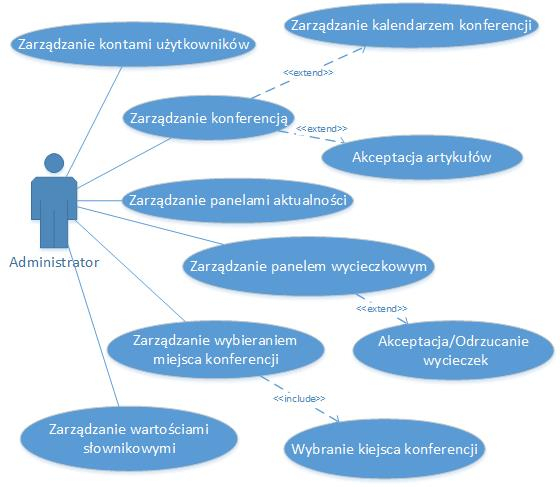
\includegraphics{administrator.jpg}
    \caption{Model diagramu przypadków użycia użytkownika administrator.}
    \label{fig:administrator}
\end{figure}

Administrator będzie pełnił rolę nadzorczą nad całym systemem. Administrator po pierwsze ma możliwość zarządzania kontami użytkowników, co roku będzie zgłaszał listę pracowników do udziału konferencji, a system za pomocą wiadomości e-mail prześle do zaproszonych wiadomość ze specjalnie spreparowanym linkiem referencyjnym który przeniesie go do systemu. Rolą administratora będzie również dodawanie listy recenzentów z której system będzie przydzielał osoby do recenzowania artykułów napisanych przez pracowników.\newline
Administrator będzie zarządzał wartościami słownikowymi systemu, czyli na przykład słownikiem możliwych specjalizacji pracowników i recenzentów, który to słownik będzie służył algorytmowi doboru recenzenta do artykułu. Również typów kont pracowniczych (na przykład: doktorant, pracownik emerytowany itp.), a także słownika kryteriów oceny (na przykład: do poprawy, może być). \newline
W panelu wycieczek administrator będzie mógł akceptować/odrzucać pomysły wycieczek dodawanych przez zarządcę wycieczek, od momentu akceptacji wycieczki przez administratora jest ona widoczna przez innych uczestników konferencji, wcześniej nie. \newline
Administrator będzie zarządzał również przebiegiem samej konferencji. Będzie zarządzał kalendarzem konferencji tj. planował na osi czasu wystąpienia poszczególnych prelegentów i ustalał agendę konferencji. Będzie miał prawo odgórnej akceptacji artykułów, nawet takich które mają status ``do poprawy''. \newline
Administrator będzie wybierał miejsce konferencji, propozycje zgłoszone przez pracowników będą również przez nich oceniane po czym administrator podejmie decyzję które miejsce wybrać. Administrator będzie uzupełniał dane o konferencji na stronie startowej. \newline
Kolejnym zadaniem będzie zarządzanie panelem aktualności, gdzie będzie mógł dodać ważne inforamcje na temat konferencji (na przykład że konferencja będzie tydzień później, że został zmieniony hotel), przez co informacja będzie lepiej widoczna dla użytkowników.

\subsection{Pracownik}

\begin{figure}[!tb]
    \centering
    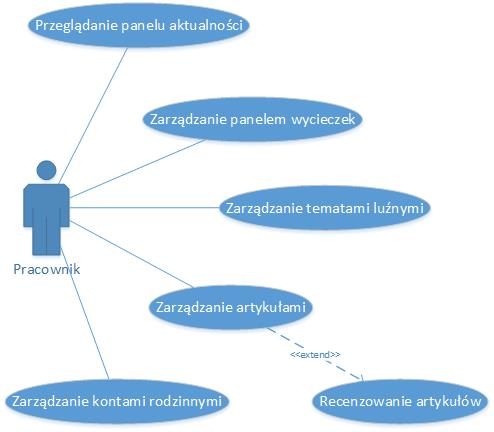
\includegraphics{pracownik.jpg}
    \caption{Model diagramu przypadków użycia użytkownika pracownik.}
    \label{fig:pracownik}
\end{figure}

Pracownik będzie miał dostęp do wszystkich paneli w systemie. Będzie mógł komentowac wycieczki i zapisywac się na nie. \newline
W panelu tematów luźnych będzie mógł dodać propozycję swojego tematu która trafi do akceptacji przez administratora, wiąże się to z tym że w szczególności przez dwóch pracowników może zostać zaproponowany podobny temat, wtedy administrator będzie mógł wstawić je do kalendarza w tym samym miejscu, albo jeden po drugim. \newline
Najbardziej rozbudowaną funkcjonalnością pracownika będzie panel zarządzania artykułami, tutaj pracowniik będzie zgłaszał temat swojego arytkułu, następnie pisał go przy użyciu odpowiedniego szablonu, później artykuł trafi do recenzenta. System będzie przydzielał do każdego artykułu recenzenta przy użyciu odpowiedniego algorytmu. \newline
Pracownikowi zostanie również dana możliwość dodania dowolnej liczby kont typu rodzina pracownika. \newline
Jedną z ważniejszych funkcjonalności pracownika jest zglaszanie propozycji miejsca konferencji, pracownik poprzez system może również komentować i oceniać propozycje konferencji innych pracowników

\subsection{Rodzina pracownika}

\begin{figure}[!tb]
    \centering
    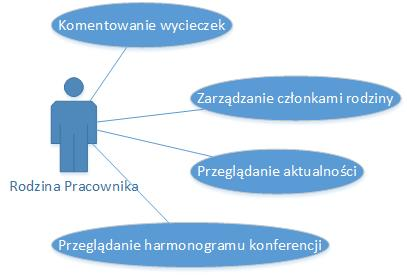
\includegraphics{rodzina.jpg}
    \caption{Model diagramu przypadków użycia użytkownika rodzina pracownika.}
    \label{fig:rodzina}
\end{figure}

Użytkownik konta rodzina pracownika będzie miał dostęp do modułu wycieczkowego, podgląd panelu aktualności, strony głównej konferencji, oraz harmonogramu konferencji . \newline
Najciekawszym panelem dla rodziny pracownika będzie moduł wycieczkowy, gdzie będzie mógł komentować wycieczki, będzie miał również możliwość zgłoszenia chęci udziału w wycieczkach.

\subsection{Zarządca wycieczek}

\begin{figure}[!tb]
    \centering
    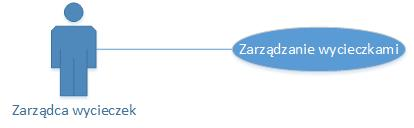
\includegraphics{zarzadcawycieczek.jpg}
    \caption{Model diagramu przypadków użycia roli zarządca wycieczek.}
    \label{fig:zarzadcawycieczek}
\end{figure}

Rola ta może zostać nadana komuś z grona pracowników. Zadaniem tej osoby będzie zgłaszanie wycieczek które będą następnie przechodziły do akceptacji przez administratora i będą widoczne w panelu wycieczkowym. Będzie odpowiedzialny za aktualizację informacji. Jego rolą będzie również dodawanie lokalów gastronomicznych, atrakcji turystycznych oraz placówek medycznych w miejscu konferencji.

\subsection{Recenzent}

\begin{figure}[!tb]
    \centering
    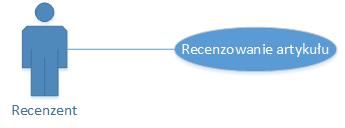
\includegraphics{recenzent.jpg}
    \caption{Model diagramu przypadków użycia użytkownika recenzent.}
    \label{fig:recenzent}
\end{figure}

Będzie to osoba która nie będzie brała udziału w konferencji, będzie jedynie recenzowała artykuł pracownika. Będzie przydzielany do artykułu przez system który za pomoca dopasowania specjalności recenzenta do tematyki artykułu znajdzie najlepszego kadydata do recenzowania. Recenzent nie będzie nic wiedział o autorze artykułu który recenzuje.

\section{Historia Zmian}

\begin{tabularx}{\textwidth}{X|l|X}
\hline
\textbf{Data zmiany} & \textbf{Kto zmienił} & \textbf{Co zostało zmienione} \\ \hline
11 mar 2015          & Błądek Piotr         & Utworzenie dokumentu          \\ \hline
11 mar 2015          &Błądek Piotr          &  Dodanie historii zmian            \\ \hline
13 mar 2015          &Błądek Piotr          &  Dodanie dokumentów powiązanych i przypadków użycia            \\ \hline
13 mar 2015          &Błądek Piotr          &  Dodanie spisu rysunków            \\ \hline
29 mar 2015          &Błądek Piotr          &  Dodanie nowych ról, aktualizacja istniejących            \\ \hline
\end{tabularx}